\documentclass[notes,11pt,aspectratio=169,xcolor=table]{beamer}

\usepackage{pgfpages}
\setbeameroption{hide notes} % Only slides
% \setbeameroption{show only notes}  % Only notes
% \setbeameroption{show notes on second screen=right} % Both

\usepackage{helvet}
\usepackage[default]{lato}
\usepackage{array}
\usepackage{minted}
\usepackage{tikz}
\usetikzlibrary{shapes.geometric,positioning,snakes,calc,arrows,decorations.markings,shapes.misc,matrix,fit,tikzmark}
\usepackage{pgfplots}
\pgfplotsset{compat=1.18}
\usepackage{graphicx,verbatim}
\usepackage{amsmath,mathpazo,hyperref,lipsum,multirow,dcolumn,bbm,booktabs}
\usepackage[style=authoryear,sorting=nyt,uniquename=false]{biblatex}
\addbibresource{references.bib}

\setbeamertemplate{note page}{\pagecolor{yellow!5}\insertnote}
\newtheorem{proposition}{Proposition}
\newcolumntype{d}[0]{D{.}{.}{5}}

% Colors
\definecolor{blue}{RGB}{0,114,178}
\definecolor{red}{RGB}{213,94,0}
\definecolor{yellow}{RGB}{240,228,66}
\definecolor{green}{RGB}{0,158,115}
\definecolor{MyBackground}{RGB}{255,253,218}

% Theme tweaks
\hypersetup{colorlinks=false, linkbordercolor=white, linkcolor=blue}
\setbeamercolor{frametitle}{fg=blue}
\setbeamercolor{title}{fg=blue}
\setbeamertemplate{footline}[frame number]
\setbeamertemplate{navigation symbols}{}
\setbeamertemplate{itemize items}{-}
\setbeamercolor{itemize item}{fg=blue}
\setbeamercolor{itemize subitem}{fg=blue}
\setbeamercolor{enumerate item}{fg=blue}
\setbeamercolor{enumerate subitem}{fg=blue}
\setbeamercolor{button}{bg=MyBackground,fg=blue}
\setbeamercolor{section in toc}{fg=blue}
\setbeamercolor{subsection in toc}{fg=red}
\setbeamersize{text margin left=1em,text margin right=1em}

\newenvironment{wideitemize}{\itemize\addtolength{\itemsep}{10pt}}{\enditemize}

% Optional transition slide background
\newenvironment{transitionframe}{
  \setbeamercolor{background canvas}{bg=yellow}
  \begin{frame}}{\end{frame}}

% Title
\title[]{International Trade: Data Lab — Solving the Heckscher–Ohlin Model}
\subtitle[]{Your first general-equilibrium price–factor-price solver}
\author[Góes]{Carlos Góes\inst{1}}
\date{Fall 2025}
\institute[GWU]{\inst{1} George Washington University}

\begin{document}

%----------------------------------------%
% Title
%----------------------------------------%
\frame{\titlepage}
\addtocounter{framenumber}{-1}

%----------------------------------------%
\section{Goals \& Roadmap}

\begin{frame}{Plan for today}
\begin{wideitemize}
  \item Recap HO building blocks: zero-profit, factor demands, full-employment
  \item Map theory to a computable system: \(p \leftrightarrow \omega \equiv w/r\)
  \item Build functions for \(RS(p)\), \(RD(p)\), and \(ED(p)=RS-RD\)
  \item Safely bracket the root (log grid), then solve with bisection
  \item Plot checks, interpret \(p^\*,\omega^\*\), and run comparative statics
\end{wideitemize}
\note{We’ll follow the exact structure of our small solver: price-to-factor price mapping,
then RS/RD, then ED root-finding, then plots.}
\end{frame}

%----------------------------------------%
\section{Model Recap (HO)}

\begin{frame}{Two goods, two factors, two countries}
\begin{wideitemize}
  \item Goods: \(C\) (cloth), \(T\) (technology or “machines”); Factors: \(K\), \(L\)
  \item Production in each country \(i\): Cobb–Douglas
  \[
    Y_g = Z_g K_g^{\beta_g} L_g^{1-\beta_g},\qquad g\in\{C,T\},\quad Z_g=1 \text{ for lab}
  \]
  \item Unit cost: \(c_g(w,r)=\dfrac{w^{1-\beta_g} r^{\beta_g}}{(1-\beta_g)^{1-\beta_g}\beta_g^{\beta_g}}\)
  \item Zero-profit: \(p_g=c_g(w,r)\). Taking the ratio gives
  \[
  \frac{p_C}{p_T}=\Phi\,\omega^{\,\beta_T-\beta_C},\quad \omega \equiv \frac{w}{r},\quad 
  \Phi=\frac{(1-\beta_T)^{1-\beta_T}\beta_T^{\beta_T}}{(1-\beta_C)^{1-\beta_C}\beta_C^{\beta_C}}
  \]
\end{wideitemize}
\note{This maps the relative commodity price \(p\equiv p_C/p_T\) to factor price ratio \(\omega=w/r\).}
\end{frame}

\begin{frame}{Allocations and outputs in a country}
\begin{wideitemize}
  \item With \(\omega\) known from \(p\), full-employment and factor cost shares imply
  \[
  L_C = \frac{K - a_T\,\omega\,L}{(a_C-a_T)\,\omega},\quad L_T=L-L_C,\qquad 
  a_g\equiv \frac{\beta_g}{1-\beta_g}
  \]
  \item Outputs (per country):
  \[
   Y_C=(a_C\omega)^{\beta_C} L_C, \qquad Y_T=(a_T\omega)^{\beta_T} L_T
  \]
  \item Aggregate across \(H\) and \(F\) to get world \(Y_C,Y_T\) and relative supply \(RS=Y_C/Y_T\).
\end{wideitemize}
\note{These are the exact formulas used in the code for speed and transparency.}
\end{frame}

%----------------------------------------%
\section{From Theory to Code}

\begin{frame}[fragile=singleslide]{Parameterization}
\begin{minted}{python}
# Preferences and technology (lab defaults)
beta_C, beta_T = 1/3, 2/3
alpha_H, alpha_F = 0.5, 0.5         # Cobb-Douglas final demand shares

# Endowments
K_H, L_H = 4.0, 8.0
K_F, L_F = 3.0, 2.0

# Convenience
a_C = beta_C / (1 - beta_C)
a_T = beta_T / (1 - beta_T)
Phi = ((1 - beta_T)**(1 - beta_T) * beta_T**beta_T) / \
      ((1 - beta_C)**(1 - beta_C) * beta_C**beta_C)
\end{minted}
\note{Same primitives as in the attached script.}
\end{frame}

\begin{frame}[fragile=singleslide]{Price $\leftrightarrow$ Factor Price}
\begin{minted}{python}
def omega_of_p(p: float) -> float:
    # p = Phi * omega^(beta_T - beta_C)
    exponent = 1.0 / (beta_T - beta_C)
    return (p / Phi) ** exponent
\end{minted}

\begin{minted}{python}
def L_C_country(omega: float, K_i: float, L_i: float) -> float:
    # L_C = (K - a_T * omega * L) / ((a_C - a_T) * omega)
    return (K_i - a_T * omega * L_i) / ((a_C - a_T) * omega)
\end{minted}
\note{Both formulas come straight from zero-profit + full employment.}
\end{frame}

\begin{frame}[fragile=singleslide]{World Relative Supply and Demand}
\begin{minted}{python}
def RS_world(p: float) -> float:
    w_over_r = omega_of_p(p)
    # Home
    LcH = L_C_country(w_over_r, K_H, L_H); LtH = L_H - LcH
    YcH = (a_C * w_over_r)**beta_C * LcH
    YtH = (a_T * w_over_r)**beta_T * LtH
    # Foreign
    LcF = L_C_country(w_over_r, K_F, L_F); LtF = L_F - LcF
    YcF = (a_C * w_over_r)**beta_C * LcF
    YtF = (a_T * w_over_r)**beta_T * LtF
    return (YcH + YcF) / (YtH + YtF)
\end{minted}

\begin{minted}{python}
def RD_world(p: float) -> float:
    w_over_r = omega_of_p(p); w = w_over_r; r = 1.0
    YH = w*L_H + r*K_H; YF = w*L_F + r*K_F
    Gamma = (alpha_H*YH + alpha_F*YF) / ((1-alpha_H)*YH + (1-alpha_F)*YF)
    return Gamma / p
\end{minted}
\note{RD comes from Cobb-Douglas final demand with world income weights.}
\end{frame}

\begin{frame}[fragile=singleslide]{Excess Demand and Solver}
\begin{minted}{python}
def excess_demand(p: float) -> float:
    return RS_world(p) - RD_world(p)
\end{minted}

\begin{minted}{python}
import numpy as np, math

def find_bracket(f, p_min=1e-4, p_max=1e4, points=1000, max_tries=4):
    for _ in range(max_tries):
        xs = np.logspace(math.log10(p_min), math.log10(p_max), points)
        vals = np.sign([f(x) for x in xs])
        flips = vals[:-1] * vals[1:] < 0
        idx = np.where(flips)[0]
        if idx.size:
            i = idx[0]; return xs[i], xs[i+1]
        points *= 2
    raise RuntimeError("No bracket found; widen search.")
\end{minted}

\begin{minted}{python}
def bisection(f, low, high, tol=1e-9, max_iter=200):
    fl, fh = f(low), f(high)
    if fl * fh > 0:
        raise ValueError("Root not bracketed.")
    for _ in range(max_iter):
        mid = 0.5*(low + high); fm = f(mid)
        if abs(fm) < tol or (high - low) < tol: return mid
        if fl * fm < 0: high, fh = mid, fm
        else: low, fl = mid, fm
    raise RuntimeError("No convergence.")
\end{minted}
\note{Log-grid bracketing prevents runaway price guesses; bisection gives robustness.}
\end{frame}

\begin{frame}[fragile=singleslide]{Compute \(\;p^\*\) and \(\omega^\*\)}
\begin{minted}{python}
low, high = find_bracket(excess_demand)
p_star = bisection(excess_demand, low, high)
omega_star = omega_of_p(p_star)
print(f"p* = {p_star:.6f},  omega* = {omega_star:.6f}")
\end{minted}

\begin{minted}{python}
# Plot ED and mark the root
import matplotlib.pyplot as plt
xs = np.linspace(0.5, 1.5, 400)
ys = [excess_demand(x) for x in xs]
fig, ax = plt.subplots(figsize=(9,5.2))
ax.plot(xs, ys, linewidth=2)
ax.axhline(0, color='black', linewidth=1)
ax.axvline(p_star, color='black', linestyle='--')
ax.set_xlabel(r"Relative price $p \equiv p_C/p_T$")
ax.set_ylabel(r"ED$(p)=RS(p)-RD(p)$")
ax.set_title("Excess Demand and Equilibrium")
plt.show()
\end{minted}
\note{Always inspect ED visually; monotonicity ensures a unique intersection.}
\end{frame}

%----------------------------------------%
\section{Graphics: RS \& RD}

\begin{frame}{World Trade Equilibrium (schematic)}
\centering
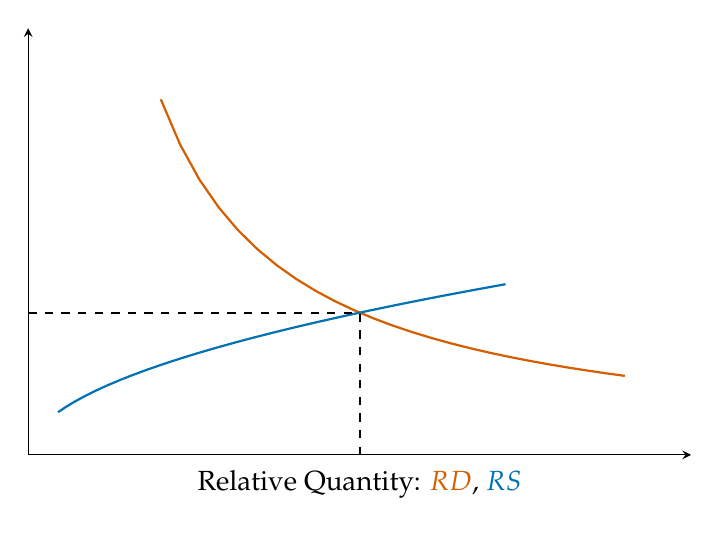
\begin{tikzpicture}
\begin{axis}[
  xlabel={Relative Quantity: \textcolor{red}{$RD$}, \textcolor{blue}{$RS$}},
  ymin=0, ymax=3, xmin=0, xmax=2,
  ytick=\empty, xtick=\empty,
  axis lines=left, width=10cm, height=7cm
]
\addplot[domain=0.4:1.8, thick, red] (x, {1.0/x}); % RD ~ 1/p over Q
\addplot[domain=0.3:1.2, thick, blue] ({x^(2/1)}, x); % stylized upward RS
\addplot[dashed, thick] coordinates {(0,1) (1,1)};
\addplot[dashed, thick] coordinates {(1,0) (1,1)};
\node[anchor=east] at (axis cs:0,1) {\scriptsize $p^{*}$};
\end{axis}
\end{tikzpicture}
\note{Stylized: RD downward (in p), RS upward (in p). Intersection pins $p^*$ and $Q$ ratio.}
\end{frame}

%----------------------------------------%
\section{Comparative Statics}

\begin{frame}{What moves $p^*$ and $\omega^*$?}
\begin{wideitemize}
  \item Endowments: \(\uparrow K_H\) or \(\uparrow K_F\) shifts world RS toward \(C\) if \(C\) is capital intensive
  \item Technology shares: \(\uparrow \beta_C\) (more capital intensive \(C\)) steepens RS
  \item Preferences: \(\uparrow \alpha\) raises RD at given \(p\), pushing \(p^*\) up
  \item \textbf{Stolper–Samuelson:} \(\uparrow p_C\) \(\Rightarrow\) \(\uparrow \omega=w/r\) if \(C\) is labor- or capital-intensive depending on \(\beta\)
  \item \textbf{Rybczynski:} At fixed prices, factor growth expands output of the factor-intensive sector
\end{wideitemize}
\note{Use the code to flip signs and confirm factor price responses numerically.}
\end{frame}

\begin{frame}[fragile=singleslide]{Quick comparative statics (live toggle)}
\begin{minted}{python}
def solve_and_report(KH, LH, KF, LF, bC, bT, aH=0.5, aF=0.5):
    global K_H, L_H, K_F, L_F, beta_C, beta_T, a_C, a_T, Phi, alpha_H, alpha_F
    K_H, L_H, K_F, L_F = KH, LH, KF, LF
    beta_C, beta_T = bC, bT
    alpha_H, alpha_F = aH, aF
    a_C = beta_C/(1-beta_C); a_T = beta_T/(1-beta_T)
    Phi = ((1-beta_T)**(1-beta_T) * beta_T**beta_T) / \
          ((1-beta_C)**(1-beta_C) * beta_C**beta_C)
    lo, hi = find_bracket(excess_demand)
    pstar = bisection(excess_demand, lo, hi)
    omegastar = omega_of_p(pstar)
    print(f"p*={pstar:.4f},  w/r={omegastar:.4f}")
\end{minted}
\end{frame}

%----------------------------------------%
\section{Exercises}

\begin{frame}{Exercises (to submit)}
\begin{wideitemize}
  \item \textbf{E1.} Starting from the baseline, double \(K_H\). Report \((p^\*,\omega^\*)\) and interpret.
  \item \textbf{E2.} Make \(C\) more capital intensive (\(\beta_C=0.5\), \(\beta_T=0.5\)). What happens to RS and to \((p^\*,\omega^\*)\)?
  \item \textbf{E3.} Shift preferences to \(\alpha_H=\alpha_F=0.6\). Show the RD shift and solve again.
  \item \textbf{E4.} Verify Stolper–Samuelson numerically by shocking \(p\) and backing out \(\omega\) via \(\omega(p)\).
\end{wideitemize}
\note{Turn in a short note with one figure per exercise and one paragraph of interpretation.}
\end{frame}


\end{document}
